%DIF PREAMBLE EXTENSION ADDED BY LATEXDIFF
%DIF UNDERLINE PREAMBLE %DIF PREAMBLE
\RequirePackage[normalem]{ulem} %DIF PREAMBLE
\RequirePackage{color}\definecolor{RED}{rgb}{1,0,0}\definecolor{BLUE}{rgb}{0,0,1} %DIF PREAMBLE
\providecommand{\DIFadd}[1]{{\protect\color{blue}\uwave{#1}}} %DIF PREAMBLE
\providecommand{\DIFdel}[1]{{\protect\color{red}\sout{#1}}}                      %DIF PREAMBLE
%DIF SAFE PREAMBLE %DIF PREAMBLE
\providecommand{\DIFaddbegin}{} %DIF PREAMBLE
\providecommand{\DIFaddend}{} %DIF PREAMBLE
\providecommand{\DIFdelbegin}{} %DIF PREAMBLE
\providecommand{\DIFdelend}{} %DIF PREAMBLE
%DIF FLOATSAFE PREAMBLE %DIF PREAMBLE
\providecommand{\DIFaddFL}[1]{\DIFadd{#1}} %DIF PREAMBLE
\providecommand{\DIFdelFL}[1]{\DIFdel{#1}} %DIF PREAMBLE
\providecommand{\DIFaddbeginFL}{} %DIF PREAMBLE
\providecommand{\DIFaddendFL}{} %DIF PREAMBLE
\providecommand{\DIFdelbeginFL}{} %DIF PREAMBLE
\providecommand{\DIFdelendFL}{} %DIF PREAMBLE
%DIF END PREAMBLE EXTENSION ADDED BY LATEXDIFF

%\documentclass{sigplanconf}
%\nocaptionrule

% \documentclass[twocolumn,9pt]{article}
% \documentclass[twocolumn,10pt]{acm_proc_article-sp}

% \documentclass{acm_proc_article-sp}
\documentclass[10pt]{sigplanconf}

\conferenceinfo{PPoPP~'14}{February 15--19, 2014, Orlando, Florida, USA} 
\copyrightyear{2014} 
\copyrightdata{978-1-4503-2656-8/14/02} 

%10.1145/ 

\doi{2555243.2555244} 
% **insert the doi number of your paper from the confirmation 
% email from rightsreview@acm.org


\date{} % \vspace*{-0.2in}}

% Make sure to put back

\newcommand{\punt}[1]{}

\usepackage{endnotes,xspace}

\newcommand{\footnotenonumber}[1]{{\def\thempfn{}\footnotetext{\small #1}}}
%\usepackage[normalem]{ulem}
\usepackage{graphicx}
\usepackage{pifont}
\usepackage{mathptmx} % rm & math
\usepackage[scaled=0.90]{helvet} % ss
\usepackage{courier} % tt
% \normalfont
\usepackage[T1]{fontenc}

% \usepackage{lmodern}
% \usepackage{times}
\usepackage{subfigure}
\usepackage[hyphens]{url}
\urlstyle{rm}
\usepackage[
      colorlinks=false, %no frame around URL
      urlcolor=black, %no colors
      menucolor=black, %no colors
      linkcolor=black, %no colors
      pagecolor=black, %no colors
      breaklinks=true, %Divided a link possibly
]{hyperref}

\usepackage{color}
\usepackage{listings}
\usepackage{amsmath}
\usepackage{amsfonts}
\usepackage{amssymb}
\usepackage{comment}
\usepackage{setspace}
\usepackage{graphicx, subfigure}
\singlespacing
%\onehalfspacing
\newtheorem{thm}{Theorem}
\newtheorem{prop}[thm]{Proposition}
\newtheorem{cor}[thm]{Corollary}
\newtheorem{lem}[thm]{Lemma}
\newtheorem{defn}[thm]{Definition}

\newcommand{\cfunction}[1]{{\bf \tt #1}}
\newcommand{\malloc}{\cfunction{malloc}}
\newcommand{\realloc}{\cfunction{realloc}}
\newcommand{\free}{\cfunction{free}}
\newcommand{\madvise}{\cfunction{madvise}}
\newcommand{\brk}{\cfunction{brk}}
\newcommand{\sbrk}{\cfunction{sbrk}}
\newcommand{\mmap}{\cfunction{mmap}}
\newcommand{\munmap}{\cfunction{munmap}}
\newcommand{\mprotect}{\cfunction{mprotect}}
\newcommand{\mlock}{\cfunction{mlock}}
\newcommand{\cmark}{\ding{52}} 
\newcommand{\xmark}{\ding{53}}

\hyphenation{Heap-Layers}

\hyphenation{pthread-create}
\hyphenation{pthread-self}
\hyphenation{pthread-mutex-lock}
\hyphenation{pthread-mutex-unlock}

\newcommand{\CC}[1]{{\large \textbf{\color{red}CC:} \emph{#1} \newline}}
\newcommand{\Sheriff}{{\scshape Sheriff}}
\newcommand{\sheriff}{{\scshape Sheriff}}
\newcommand{\Predator}{{\scshape Predator}}
\newcommand{\predator}{{\scshape Predator}}
\newcommand{\pthreads}{\texttt{pthreads}}

\lstdefinelanguage{c++threads}[]{c++}{morekeywords={pthread_create,pthread_join}}

\lstset{language=c++threads, basicstyle=\ttfamily\scriptsize,frame=trbl,tabsize=4} % ,numbers=left,numberstyle=\tiny}

\definecolor{Gray}{cmyk}{0,0,0,0.5}

\begin{document}


\title{\Predator{}: Predictive False Sharing Detection}

\authorinfo{Tongping Liu}
           {School of Computer Science \\
           University of Massachusetts Amherst}
           {tonyliu@cs.umass.edu}
\authorinfo{Chen Tian \and Ziang Hu}
           {Huawei US R\&D Center}
           {Chen.Tian@huawei.com, Ziang.Hu@huawei.com}
\authorinfo{Emery D. Berger}
           {School of Computer Science \\
             University of Massachusetts Amherst}
           {emery@cs.umass.edu}

\maketitle

\begin{abstract}
False sharing is a notorious problem for multithreaded applications
that can drastically degrade both performance and
scalability. Existing approaches can precisely identify
the sources of false sharing, but only report false
sharing actually observed during execution; they do not generalize
across executions. Because false sharing is extremely sensitive to
object layout, these detectors can easily miss false sharing problems
that can arise due to slight differences in memory allocation order or
object placement decisions by the compiler. In addition, they cannot
predict the impact of false sharing on hardware with different cache
line sizes.

This paper presents \Predator{}, a predictive software-based false
sharing detector. \Predator{} generalizes from a single execution to
precisely predict false sharing that is latent in the current
execution. \predator{} tracks accesses within a range that could lead
to false sharing given different object placement. It also tracks
accesses within
\emph{virtual cache lines}, contiguous memory ranges that span actual
hardware cache lines, to predict sharing on hardware platforms with
larger cache line sizes. For each, it reports the exact program
location of predicted false sharing problems, ranked by their
projected impact on performance. We evaluate \Predator{} across a
range of benchmarks and actual applications. \Predator{} identifies
problems undetectable with previous tools, including two
previously-unknown false sharing problems, with no false
positives. \Predator{} is able to immediately locate false sharing problems in MySQL and the
Boost library that had eluded detection for years.
\end{abstract}

\section{Introduction}
\label{sec:intro} 

While writing correct multithreaded programs is often challenging,
making them scale can present even greater obstacles. Any contention can impair scalability or even cause
applications to run slower as the number of threads increases.

False sharing is a particularly insidious form of contention.
It occurs when two threads update logically-distinct objects that happen to reside on the same cache line. The resulting
coherence traffic can degrade performance by an order of
magnitude~\cite{falseshareeffect}. Unlike sources of contention like locks, false sharing is often invisible in the source code, making it difficult to find.

As cache lines have grown larger and multithreaded applications have
become commonplace, false sharing has become an increasingly important
problem. Performance degradation due to false sharing has been detected across the software stack,
including inside the Linux kernel~\cite{OSfalsesharing}, the Java
virtual machine~\cite{JVMfalsesharing}, common
libraries~\cite{libfalsesharing} and widely-used
applications~\cite{mysql,appfalsesharing}.

Recent work on false sharing detection falls short in several dimensions. Some introduce excessive performance overhead, making them impractical~\cite{falseshare:binaryinstrumentation1,falseshare:binaryinstrumentation2,falseshare:simulator}. Most do not report false sharing precisely and accurately~\cite{falseshare:binaryinstrumentation1,detect:ptu,detect:intel,falseshare:binaryinstrumentation2,DProf,qinzhaodetection}, and some require special OS support or only work on a restricted class of applications~\cite{OSdetection,sheriff}.

In addition, all of these systems share one key limitation: they can
only report \emph{observed} cases of false sharing. As Nanavati et al.\ point out, false sharing is sensitive to where objects are placed in cache lines and so can be affected by a wide range of factors~\cite{OSdetection}. For example, using the gcc compiler \emph{accidentally} eliminates false sharing in the Phoenix linear\_regression benchmark at certain optimization levels, while LLVM does not do so at any optimization level.  A slightly different memory allocation sequence (or different memory allocator) can reveal or hide
false sharing, depending on where objects end up in memory; using a different hardware platform with different addressing or cache line sizes can have the same effect. All of this means that existing tools cannot root out potentially devastating cases of false sharing that could arise with different inputs, in different execution environments, and on different hardware platforms.

This paper makes the following contributions:

\begin{itemize}

\item
\textbf{Predictive False Sharing Detection:} This paper introduces \emph{predictive false sharing analysis}, an approach that can \emph{predict} potential false sharing that does not manifest in a given run but may appear---and greatly degrade application performance---in a slightly different execution environment. 
Predictive false sharing detection thus overcomes a key limitation of previous detection tools.

\item
\textbf{A Practical and Effective Predictive False Sharing Detector:} 
This paper presents \Predator{}, a prototype predictive false sharing detector that combines compiler-based instrumentation with a runtime system. \Predator{} not only \emph{detects} but also \emph{predicts} potential false sharing problems.
\Predator{} operates with reasonable overhead (average: $6\times$ performance, $2\times$ memory). It is the first false sharing tool able to automatically and precisely uncover
false sharing problems in real applications, including 
MySQL and the Boost library.

\end{itemize}

\section{False Sharing Detection}
\label{sec:detection}

We first describe \Predator{}'s false sharing detection mechanism, which comprises both compiler and runtime system
components. Section~\ref{sec:prediction} then explains how \Predator{} predicts potential false sharing based on a single execution.

\subsection{Overview}
\label{sec:overview}

False sharing occurs when two threads
simultaneously access logically independent data in the same cache line, and where at least one of the accesses is a write.
For the purposes of exposition, we assume that each thread runs on a distinct core with its own private cache.

We observe that 
if a thread writes a cache line after other threads have 
accessed the same cache line, this write operation most likely causes at least one cache invalidation. It is this invalidation traffic that leads to performance degradation due to false sharing. To identify the root cause of such traffic due to false sharing, \Predator{} tracks cache invalidations of all cache lines, and ranks the severity of performance degradation of any detected false sharing problems according to the number of cache invalidations. 
 

% The design tradeoff of choosing compiler instrumentation has been discussed in Section~\ref{sec:instrumentationtradeoff}. 

To track cache invalidations, \Predator{} relies on compiler instrumentation to track accesses to memory. While a compiler can easily identify read or write accesses, it cannot know how and when those instructions are being executed, since that depends on a specific execution, input, and runtime environment.

Therefore, \Predator{} combines compiler instrumentation with a runtime system to track cache invalidations. The compiler
instruments memory accesses with calls to the runtime system that notify it when an access occurs (see Section~\ref{sec:compiler}), and the runtime system collects and analyzes these accesses to detect and report false sharing (see Section~\ref{sec:runtime}).

\subsection{Compiler Instrumentation}
\label{sec:compiler}

\Predator{} relies on LLVM to perform instrumentation at the intermediate representation level~\cite{llvm}.
It traverses all functions one by one and searches for memory accesses to global and heap variables.  For each memory access, \Predator{} inserts a function call to invoke the runtime system with the memory access address and access type (read or write). \Predator{} currently omits accesses to stack variables by default because stack variables are normally used for thread local storage and therefore do not normally introduce false sharing. However, instrumentation on stack variables
can always be turned on if desired.

The instrumentation pass is placed at the very end of the LLVM
optimization passes so that only those memory accesses surviving all previous LLVM optimization passes are instrumented.  This technique, which can drastically reduce the number of instrumentation calls, is similar to the one used by AddressSanitizer~\cite{Addresssanitizer}.

\subsection{Runtime System}
\label{sec:runtime}

\Predator{}'s runtime system collects every memory access via the functions calls inserted by the compiler's instrumentation phase. It analyzes possible cache invalidations due to possibly interleaved reads and writes. Finally, \Predator{} precisely reports any performance-degrading false sharing problems it finds.  For global variables involved in false sharing, \Predator{} reports their name, address and size; for heap
objects, \Predator{} reports the callsite stack for their allocations, their address and size. In addition, \Predator{} provides word granularity access information for those cache lines involved in false sharing, including which threads accessed which words.  This information can further help users diagnose and fix false sharing instances.

\subsubsection{Tracking Cache Invalidations}
\Predator{} only reports those global variables or heap objects on cache lines with a large number of cache invalidations. It is critical that \Predator{} track cache invalidations precisely in order to provide accurate reports of the location of false sharing instances.
\Predator{} achieves this goal by maintaining a two entry cache history table for every cache line.  In this table,
each entry has two fields: the thread ID and access type (read or write). The thread ID is used to identify the origin of each access. As stated earlier, only accesses from different threads can cause cache invalidations.

For every new access to a cache line $L$, \Predator{} checks $L$'s history table $T$ to decide whether there is a cache invalidation based on the following rules.  Note that table $T$ only has two statuses: full and not full.  There is no ``empty'' status since every cache invalidation should replace this table with the current write access.

\begin{itemize}
\item
For each read access $R$, 
\begin{itemize}
\item
If $T$ is full, there is no need to record this read access.
\item
If $T$ is not full and another existing entry has a different thread
ID, then \Predator{} records this read and its thread by adding a new entry to the table. 
\end{itemize}
\item
For each write access $W$, 
\begin{itemize}
\item
If $T$ is full, then $W$ can cause a cache invalidation since at least one of two existing entries has a different thread ID.
After recording this invalidation, \Predator{} updates the
existing entry with $W$ and its thread.
\item
If $T$ is not full,
\Predator{} checks whether $W$ and the existing entry have the same thread ID. If
so, $W$ cannot cause a cache invalidation, so \Predator{} updates the existing
entry with $W$. Otherwise, \Predator{} identifies an invalidation on this line caused by $W$. 
After recording this invalidation information, \Predator{} updates the
existing entry with $W$ and its thread.
\end{itemize}
\end{itemize}

\subsubsection{Reporting False Sharing}

Once cache lines with many cache invalidations have been detected,
\Predator{} needs to perform further analysis to differentiate actual false sharing from true sharing. 
True sharing, e.g., multiple threads updating the same counter in a cache line, can also cause many cache invalidations.

In order to report false sharing precisely and accurately,  
\Predator{} employs the following mechanisms:

\paragraph{Distinguishing False from True Sharing.} \Predator{} keeps track of access information for each word on those cache lines involved in false sharing: how many reads or writes to each word by which thread.  When a word is accessed by multiple threads, \Predator{} marks the origin of this word as a shared access and does not track threads for further accesses to it. This approach lets \Predator{} accurately distinguish false sharing from true sharing in the reporting phase.  It also helps diagnose where
actual false sharing occurs when there are multiple fields or multiple
objects in the same cache line, as this can greatly reduce the manual
effort required to fix the false sharing problems.

\paragraph{Callsite Tracking for Heap Objects.} In order to precisely report the origins of heap objects with false
sharing problems, \Predator{} maintains detailed information so it can report source code level information for each heap
object. To obtain callsite information, \Predator{} intercepts all memory allocations and de-allocations, and relies
on the \texttt{backtrace()} function in the \texttt{glibc} library to obtain the whole callsite stack.
\Predator{} also avoids pseudo false sharing (false positives) caused by memory reuse because it updates recording information at memory de-allocations for those objects without false sharing problems; heap objects involved in false 
sharing are never reused.

\paragraph{Optimizing Metadata Lookup.}
For every access, \Predator{} needs to look up the corresponding cache line's metadata 
in order to store detailed information or update access counters. Because this operation is so frequent,
lookups need to be very efficient.
Like 
AddressSanitizer~\cite{Addresssanitizer} and other systems~\cite{qinzhaodetection,Valgrind},
\Predator{} uses a shadow memory mechanism to store metadata for every piece of application data. 
Thus, \Predator{} can compute and locate corresponding metadata directly via address arithmetic.

\paragraph{Custom Memory Allocation.} In order to efficiently support shadow memory, \Predator{} uses a predefined starting address and fixed size for its heap.  It also contains a custom memory allocator, which is built with Heap Layers~\cite{heaplayers} using a ``per-thread-heap'' mechanism similar to that used by Hoard~\cite{Hoard}.  In this allocator, memory allocations from different threads never occupy the same physical cache line, which automatically prevents false sharing among different objects.  However, using this custom memory allocator implies that false sharing caused by a memory allocator cannot be detected by \Predator{}. It is straightforward to solve such false sharing problems by using an allocator like Hoard that avoids this kind of false sharing.


\subsection{Optimizations}
\label{optimization}
Tracking every memory access can be extremely expensive.  
\Predator{} utilizes the following mechanisms to further reduce overhead.

\subsubsection{Threshold-Based Tracking Mechanism}
\label{sec:thresholdtracking}
\Predator{} aims to detect false sharing that significantly degrades performance. Since cache invalidations are the root cause of performance degradation and only writes 
can possibly introduce cache invalidations, 
cache lines with a small number of writes are never a significant performance bottleneck.
For this reason, \Predator{} only tracks cache invalidations
once the number of writes to a cache line crosses a
pre-defined threshold, which we refer to as the {\it TrackingThreshold}. 
Until this threshold is reached, \Predator{} only tracks the number of writes on a cache line 
while skipping tracking for reads.
This mechanism reduces runtime and memory overhead
at the same time.

\Predator{} maintains two arrays in shadow memory: 
{\it CacheWrites} tracks the number of memory writes to every cache line, and
{\it CacheTracking} tracks detailed information 
for each cache line once the number of writes on a cache line exceeds
the {\it TrackingThreshold}. 
If the threshold is not reached, there is no need to check the corresponding {\it CacheTracking} entry. 

\begin{figure}[!t]
\begin{lstlisting}
void HandleAccess(unsigned long addr, bool isWrite) {
unsigned long cacheIndex = addr>>CACHELINE_SIZE_SHIFTS;
CacheTrack *track = NULL;

if (CacheWrites[cacheIndex] < TRACKING_THRESHOLD) {
if (isWrite) {
if (ATOMIC_INCR(&CacheWrites[cacheIndex]) 
>= TRACKING_THRESHOLD) {
track = allocCacheTrack();
ATOMIC_CAS(&CacheTracking[cacheIndex], 0, track));
}
} 
} else {
track = CacheTracking[index];
if (track) {
// Track cache invalidations and detailed accesses
track->handleAccess(addr, isWrite);
}
}
}
\end{lstlisting}
\caption{Pseudo-code for \Predator{}'s memory access instrumentation.\label{fig:algorithm}}
\end{figure}

To avoid expensive lock operations, \Predator{} uses atomic instruction to increment 
the {\it CacheWrites} counter for each cache line. 
Once the number of writes of a cache line reaches the predefined threshold,
\Predator{} allocates space to track detailed cache invalidations and word accesses.
\Predator{} also 
uses an atomic compare-and-swap to set the cache tracking address for this cache line in
the shadow mapping.
After {\it CacheWrites} on a cache line have crossed the {\it TrackingThreshold}, 
\Predator{} tracks all read and write accesses to this cache line.

\subsubsection{Selective Compiler Instrumentation}
\label{sec:selectinstrumentation}

\Predator{} relies on instrumentation to provide memory access information to the runtime system 
and detects false sharing based on the sequences of memory accesses to every cache line. 
The performance overhead of doing this is proportional to 
the degree of instrumentation: more 
instrumentation means higher performance overhead. \Predator{}'s design makes it possible to trade performance and accuracy as needed.

Currently, \Predator{} only adds instrumentation once for each type of memory access on each address 
in the same basic block. 
This selective instrumentation does not normally affect the effectiveness of detection. 
Because \Predator{} aims to detect cases of false sharing with many cache invalidations,
less tracking inside a basic block can induce fewer cache invalidations, 
but this does not affect the overall behavior of cache invalidations. 


To further improve performance,
\Predator{} could easily be extended to support more flexible instrumentation:
\begin{itemize}
\item
\Predator{} could selectively instrument both reads and writes or only writes.
Instrumenting only writes reduces overhead while detecting write-write false sharing, 
as \Sheriff{} does~\cite{sheriff}.
\item
\Predator{} can be set to instrument or skip specific code or data. 
For example, the user could provide a blacklist so that given modules,
functions or variables are not instrumented. 
Conversely, the user could provide a whitelist so that only specified functions or variables are instrumented. 
\end{itemize}

\subsubsection{Sampling Mechanism}
\label{sec:sample}
As Section~\ref{sec:thresholdtracking} describes, once the number of
writes on a cache line exceeds the {\it TrackingThreshold}, every
access must be tracked to store details such as word access
information, the access count, and the cache access history table
of this cache line.  When a cache line is involved in false or true
sharing, updating those counters can exacerbate the impact of sharing
on performance: not only is there an invalidation on an application
cache line, but there is also at least another cache invalidation
caused by updating the metadata of the corresponding cache lines.

To further reduce performance overhead, \Predator{} only samples the first specified
number of accesses of each sampling interval for problematic cache lines. 
Currently, \Predator{} maintains an access counter for each cache line
and only tracks the first $10,000$ out of every 1 million
accesses to a cache line (a 1\% sampling rate).

\section{False Sharing Prediction}
\label{sec:prediction}
This section further motivates predictive false sharing and explains how to support it in the runtime system.  

\subsection{Overview}
%\begin{figure*}[!htb]
\label{sec:predictoverview}

\begin{figure}[!t]
\begin{center}
\vspace{1.2em}
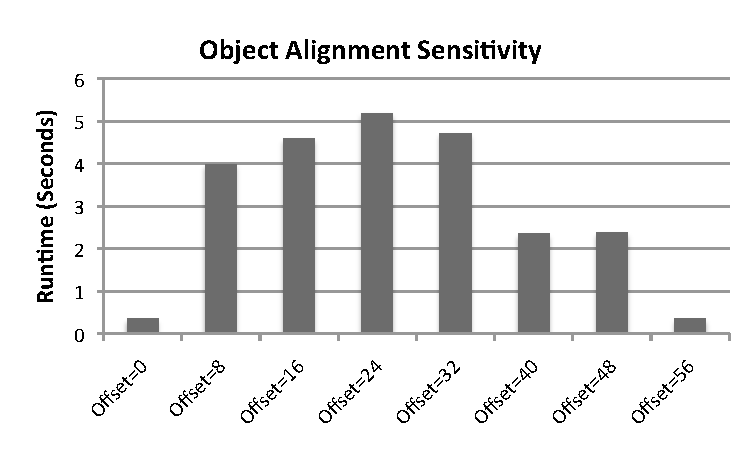
\includegraphics[width=3.3in]{fig/perfsensitive}
\vspace{1.2em}
\end{center}
\caption{
Performance of the linear\_regression benchmark from the Phoenix benchmark suite.
Performance is highly sensitive to the offset of the starting address of the (potentially) falsely-shared object 
from the start of the cache line. 
\label{fig:perfsensitive}}
\end{figure}

False sharing can depend on 
the alignment of objects and corresponding cache lines.
Figure~\ref{fig:perfsensitive} demonstrates the impact of placement on linear\_regression, a benchmark from the Phoenix benchmark suite.
For this benchmark,
when the offset of the starting address between the potentially falsely-shared object and corresponding cache lines 
is $0$ or $56$ bytes, 
there is no false sharing. 
When the offset is $24$ bytes, we see the most severe performance effect caused 
by false sharing. 
The performance difference between these two scenarios can be as great as $15\times$.

Existing detection tools only report observed false sharing.
In this case, they would miss a severe false sharing problem that could occur in the wild if the offset of the starting 
address was $0$ bytes or $56$ bytes in their test environment.
\Predator{} overcomes this shortcoming by accurately predicting potential false sharing.

\begin{figure*}
\begin{center} 
\subfigure[No false sharing]{%
\label{fig:nofs}
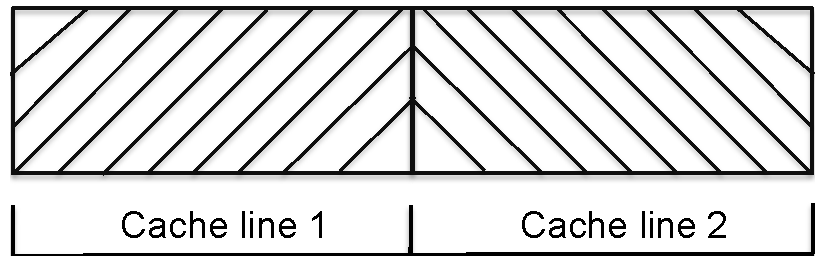
\includegraphics[width=0.24\textwidth]{fig/Potential1}
}%
\hspace{30pt}
\subfigure[False sharing with larger cache size]{%
\label{fig:fslarger}
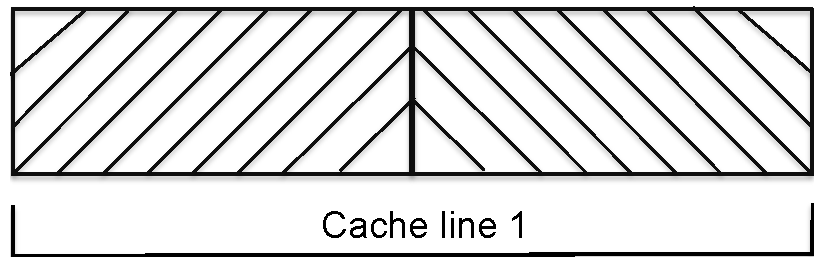
\includegraphics[width=0.24\textwidth]{fig/Potential2}
}%
\hspace{30pt}
\subfigure[False sharing with different alignment]{%
\label{fig:fsnoalignment}
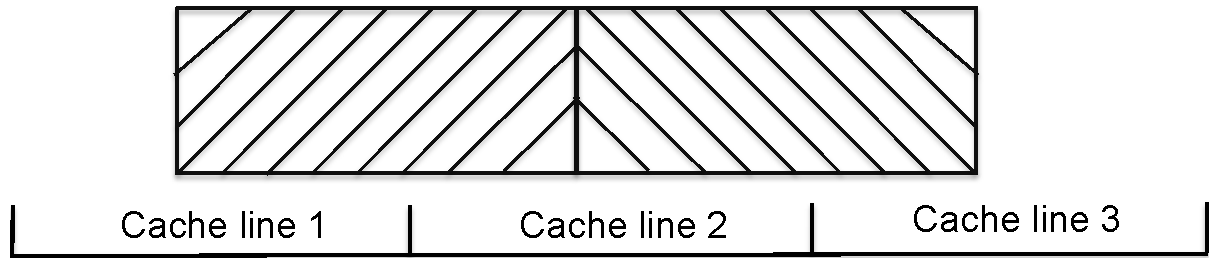
\includegraphics[width=0.36\textwidth]{fig/Potential3}
}%
\end{center}
\caption{False sharing under different scenarios (see Section~\ref{sec:predictoverview}).}
\label{fig:potentialfalsesharing}
\end{figure*}

\Predator{} predicts {\it potential false sharing}, the type of
false sharing that does not 
manifest in the current execution but may appear and greatly affect programs' performance
in a slightly different environment.

Figure~\ref{fig:potentialfalsesharing} presents a simplified overview of how false sharing can be triggered 
by different environments.
In this figure, two rectangles with different patterns
represent two portions of the same object, updated by different threads. 
In Figure~\ref{fig:nofs}), there is no false sharing when thread T1 only updates 
cache line 1 and T2 only updates cache line 2.
However, false sharing appears in each of the following cases, even with the same
access pattern:

\begin{itemize}
\item \textbf{Doubling the cache line size.} (Figure~\ref{fig:fslarger}) When the size of a
cache line doubles,
both T1 and T2 access the same cache line, leading to false sharing.

\item \textbf{Different object starting addresses.} (Figure~\ref{fig:fsnoalignment})
If the starting address of the object is not aligned with the starting address of 
the first cache line, 
T1 and T2 can update the second cache line simultaneously, 
causing false sharing. 
\end{itemize} 

\Predator{} predicts whether programs can have potential false sharing  
in either of these two scenarios. These scenarios capture the impact of any change in the execution environment, such as a different hardware platform or a different memory allocation sequence.

\subsection{Basic Prediction Workflow}
\label{sec:predictionmechanism} 

\Predator{} focuses exclusively on potential false sharing that can 
cause performance problems.
Its implementation is based on
two key observations. First, only accesses to 
adjacent cache lines can lead to potential false sharing: 
that is, they introduce cache invalidations when the cache line size
or an object's starting address changes.
Second, only when false sharing introduces a large number of cache invalidations
can it degrade performance.

Based on these two observations, \Predator{} employs 
the following workflow to detect potential false sharing.
Note that the detection optimizations listed in Section~\ref{optimization} apply directly to prediction as well.

\begin{enumerate}
\item
Track the number of writes to different cache lines. 

\item
When the number of writes to a cache line $L$ reaches {\it TrackingThreshold},
track detailed read and write accesses for every word in both cache line $L$ 
and its adjacent cache lines. 

\item
When the number of writes to a cache line $L$ crosses a second threshold (the 
{\it PredictionThreshold}), 
identify whether there exists false sharing in $L$ and its adjacent 
cache lines by analyzing word access information collected in Step 2. 
Section ~\ref{sec:evaluatingfs} describes this process.

\item
If potential false sharing is found, continue to track cache line invalidations to confirm it. Section~\ref{sec:tracking} discusses the details.

\end{enumerate}

\subsection{Searching for Potential False Sharing}
\label{sec:evaluatingfs}

To predict potential false sharing in the cases when either the hardware cache line size doubles or when object placement changes, we first 
introduce the concept of a \emph{virtual cache line}.  A virtual cache line
is a contiguous memory range that spans one or more physical cache 
lines.

Using virtual cache lines lets \Predator{} predict potential false sharing in both of the scenarios mentioned above. When the hardware cache line size doubles, a virtual line is
composed of two original contiguous cache lines and the first cache
line has an even index number.  Thus, only cache lines $2*i$ and
$2*i+1$ can form a virtual line.  To predict false sharing due to different starting
addresses, a virtual line can have the same size as physical lines,
but can be positioned arbitrarily: unlike actual cache lines, the
starting address of a virtual cache line does not need to be multiple
of the cache line size.  For instance, a 64-byte long virtual line can
consist of the range $[0,64)$ bytes or $[8,72)$ bytes.

To search for potential false sharing problems, 
\Predator{} searches for a hot access pair on line $L$ and its adjacent cache lines 
by analyzing the detailed word access information collected in Step 2. 
A hot access in a cache line refers to a word whose number of read or write accesses 
is larger than the average number of accesses to each word of cache line $L$.
For every hot access $X$ in cache line $L$, \Predator{} searches for another
hot access $Y$ in $L$'s previous cache line or next cache line satisfying
the following conditions: 
(1) $X$ and $Y$ reside in the same virtual line;
(2) at least one of $X$ or $Y$ are a write access; and 
(3) $X$ and $Y$ are issued by different threads.


Whenever it finds such a pair $X$ and $Y$, 
\Predator{} identifies potential performance-degrading false sharing whenever
the number of cache invalidations caused by $X$ and $Y$, at a possible virtual line, 
is greater than the average number of accesses on each word of $L$. 
This approach is based on a the same observation as in detection:
\emph{if a thread writes a virtual line after other threads 
have accessed the same virtual line, this write operation most likely causes at least one cache 
invalidation}. 
\Predator{} conservatively assumes that accesses from different threads occurs in an interleaved manner; that is, it assumes that the schedule exposes false sharing.
This approach ensures that \Predator{} does not miss any potential false sharing cases.

After identifying possible false sharing, \Predator{} goes to Step 4 to 
verify whether this is an actual false sharing problem.

\subsection{Verifying Potential False Sharing}
\label{sec:tracking}

\Predator{} verifies potential false sharing by tracking 
cache invalidations of a problematic virtual line.

For potential false sharing caused by double cache line size, as described in
Section~\ref{sec:evaluatingfs}, a virtual line is always composed of 
cache line with index $2*i$ and $2*i+1$. 
\Predator{} tracks cache invalidations
on the virtual line on which false sharing has been discovered.

However, for the case of a change in starting address,
two hot accesses with a distance less than the cache line size 
can form multiple virtual lines. 
There is thus an additional step required to determine which virtual line needs to be tracked.


\begin{figure}
\begin{center} 
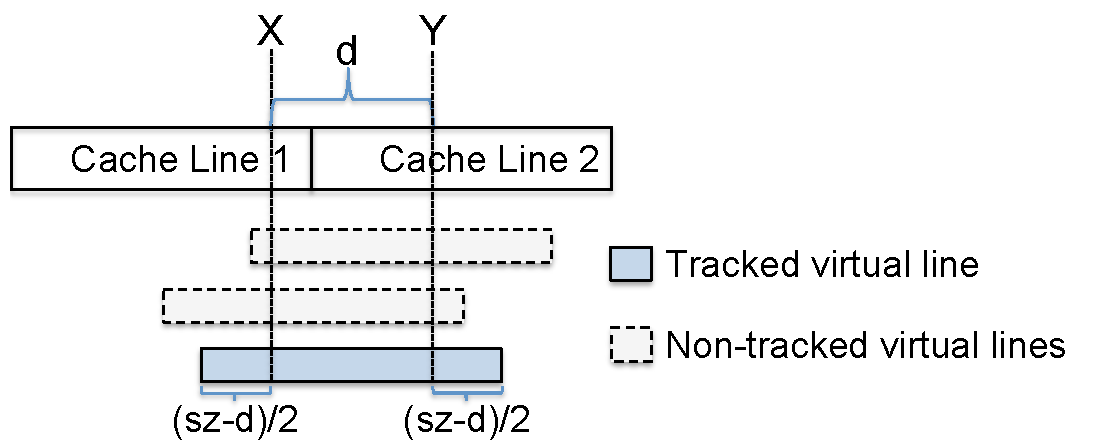
\includegraphics[width=3.3in]{fig/trackpotential}
\end{center}
\caption{Determining a virtual line with size $sz$ according to hot accesses (see Section~\ref{sec:tracking}).
\label{fig:trackpotential}}
\end{figure}

Given two words with the hot accesses shown in Figure~\ref{fig:trackpotential}, 
\Predator{} leaves the same space before $X$ and after $Y$ in determining a virtual line. 
That is, the virtual line starting 
at location $X-((sz-d)/2)$ and ending at $Y+((sz-d)/2)$ is tracked. 
This choice allows tracking more possible cache invalidations caused by
adjacent accesses to $X$ and $Y$. 
Since adjusting the starting address of a virtual line has the same effect as
adjusting the starting address of an object in detecting false sharing,
all cache lines related to the same object must be adjusted at the same time.
\Predator{} then tracks cache invalidations based on these adjusted virtual lines.

\section{Experimental Evaluation}
\begin{figure*}[htb]
{\centering
\tiny
\subfigure{\lstinputlisting[numbers=none,frame=none,boxpos=t]{fig/linearregression.report}}
\caption{An example report by \Predator{} indicating false sharing in the linear\_regression benchmark.
\label{fig:lrreport}}
}
\end{figure*}


\label{sec:evaluation}

This section answers the following questions:
\begin{itemize}
\item
How effective is \Predator{} at detecting and predicting false sharing ($\S$~\ref{sec:effective})?

\item
What is \Predator{}'s overhead, in terms of execution time ($\S$~\ref{sec:perfoverhead}) and memory ($\S$~\ref{sec:memoverhead})?

\item 
How sensitive is \Predator{} to different sampling rates ($\S$~\ref{sec:sensitivity})? 

\end{itemize}


\paragraph{Experimental Platform.} All evaluations are performed on a quiescent Intel Core 2 dual-processor system equipped with 
16GB RAM. Each processor is a 4-core 64-bit Intel Xeon running at 2.33 GHz, with a 4MB shared L2 cache and 32KB private L1 cache. The underlying operating system is an unmodified CentOS 5.5, running with Linux kernel version 2.6.18-194.17.1.el5. We use glibc version 2.5 and LLVM version 3.2. 
All applications were compiled as 64-bit executables with the optimization level set to \texttt{-O1} in order to maintain accurate source code line number information.

\paragraph{Evaluated Applications.} 
This paper evaluates two popular benchmark suites,
Phoenix (with large input)~\cite{phoenix-hpca} and PARSEC (with simlarge input)~\cite{parsec}. We were unable to include two of the benchmarks. LLVM does not compile Facesim successfully, reporting an undefined template. Canneal compiles but then aborts unexpectedly. We also evaluate \Predator{} on six real applications: MySQL, Boost, Memcached, aget, pbzip2 and pfscan.

\subsection{Detection and Prediction Effectiveness}
\label{sec:effective}

For every detected or predicted false sharing problem, \Predator{} reports source code information and detailed memory access information. Figure~\ref{fig:lrreport} shows an example for the linear\_regression benchmark. This report shows that the heap object starting with $0x40000038$ potentially causes numerous cache invalidations. The allocation callsite is provided to help locate culprits. In addition, \Predator{} also reports word-level access information of this object, which makes it possible for the developer to identify where and how false sharing occurs. From this information, we can see that this instance is a latent false sharing problem predicted by \Predator{}, since different threads are accessing different hardware cache lines.


\subsubsection{Benchmarks}
\label{sec:benchmarks}

\begin{table*}[!t]
{\centering\begin{tabular}{l|r|r|r|r|r}\hline
{\bf \small Benchmark} & {\bf \small Source Code} & {\bf \small New} & {\bf \small Without Prediction} &{\bf \small With Prediction} & {\bf \small Improvement} \\
\hline
\small \textbf{histogram} & {\small histogram-pthread.c:213} & \cmark{} &\cmark{} & \cmark{} & 46.22\%\\
\small \textbf{linear\_regression} & {\small linear\_regression-pthread.c:133} & & & \cmark{} & 1206.93\% \\
\small \textbf{reverse\_index} & {\small reverseindex-pthread.c:511} & & \cmark{} & \cmark{} & 0.09\%\\
\small \textbf{word\_count} & {\small word\_count-pthread.c:136} & & \cmark{} & \cmark{} & 0.14\%\\
\hline
\small \textbf{streamcluster} & {\small streamcluster.cpp:985} &  & \cmark{} & \cmark{} &7.52\% \\
\small \textbf{streamcluster} & {\small streamcluster.cpp:1907} & \cmark{} & \cmark{} & \cmark{} & 4.77\%\\
\hline
\end{tabular}
\caption{False sharing problems in the Phoenix and PARSEC benchmark suites. \label{table:detection}}
}
\end{table*}

Table~\ref{table:detection} provides detection results across the Phoenix and PARSEC benchmark suites. 
The first column lists the programs with false sharing problems.  The second column shows precisely where the problem is. Because all discovered false sharing occurs inside heap objects, we present callsite source code information here.  The third column, \emph{New}, indicates whether this false sharing was newly discovered by \Predator{}.  A checkmark in the following two columns indicates whether the false sharing was identified without
prediction and/or with prediction.  The final column, \emph{Improvement}, presents the performance improvement after fixing false sharing.

As the table shows, \Predator{} reveals two previously unknown false sharing problems. It is the first tool to detect false sharing problems in histogram and in line $1908$ of streamcluster. 
In histogram, multiple threads simultaneously modify different locations of the same heap object, thread\_arg\_t. 
Padding this data structure eliminates false sharing and improves performance by around 46\%. In streamcluster, multiple threads simultaneously access and update the same \texttt{bool} array, switch\_membership. Simply changing all elements of this array to a \texttt{long} type reduces the false sharing and improves performance by about 4.7\%.

%, although it is not a complete fix of false sharing. 
%None of these two false sharing problems has been reported by previous tools.
Other false sharing problems reported here were also discovered by previous work~\cite{sheriff}. We do not see significant performance improvement for the reverse\_index and word\_count benchmarks. They are reported here because the number of cache invalidations in these two programs crosses our predefined threshold.
Increasing \Predator{}'s reporting threshold would avoid reporting these cases, which are relatively insignificant.
Nonetheless, it is worth noting that these two benchmarks do indeed have false sharing problems,
which can be confirmed by the word-level information generated by \Predator{}. 

The streamcluster benchmark has another false sharing problem located at line $985$. Different threads repeatedly update the work\_mem object. The authors of streamcluster were clearly aware of this issue and provide a CACHE\_LINE macro for padding. Unfortunately, the default value of this macro is set to $32$ bytes, which is smaller than the actual cache line size of the experimental machine. Setting it to $64$ bytes instead improves performance by about 7.5\%.

The linear\_regression benchmark has an unusually severe false sharing problem. Fixing it improves performance by more than $12\times$. In this benchmark, different threads repeatedly update their thread-specific locations inside the tid\_args object inside a tight loop. Interestingly, Nanavati et al. observe that this false sharing problem occurs when using clang and disappears when using gcc with the \texttt{-O2} and \texttt{-O3} optimization levels~\cite{OSdetection}. However, we observe a different result when using our version of clang and the custom memory allocator: the false sharing problem \emph{does not occur at all} because the offset of the starting address of the potentially falsely-shared object and the start of cache line is 56 bytes (see Figure~\ref{fig:perfsensitive}). As we discuss below,\Predator{}'s prediction mechanism identifies this latent false sharing problem, highlighting the value of predictive detection.

\subsubsection{Real Applications}
We evaluate \Predator{}'s effectiveness on several widely-used real applications. These applications include a MySQL, a database server~\cite{mysql};
Boost, a standard C++ library~\cite{libfalsesharing};
Memcached, a distributed memory object caching system; aget, a download accelerator;
pbzip2, a parallel bzip2 file compressor; and pfscan, a parallel file scanner.

MySQL-5.5.32 and boost-1.49.0 are known to have false sharing problems. The other applications we examine (memcached-1.4.15, aget-0.4.1 and pbzip2-1.1.6) do not have  any known false sharing problems.

MySQL's false sharing problem caused a significant scalability problem and was very difficult to identify.
According to the architect of MySQL, Mikael Ronstrom, ``we had gathered specialists on InnoDB..., participants from MySQL support... and a number of generic specialists on 
computer performance...'', ``[we] were able to improve MySQL performance by 6$\times$ with those scalability fixes''~\cite{mysql}. 
The false sharing inside Boost is caused by the usage of a spinlock pool. Different threads may utilize different spinlocks located in the same cache line in this case. Fixing it brings a 40\% performance improvement.
\Predator{} is able to pinpoint the false sharing locations in both MySQL and the Boost library. 
For the other four applications, \Predator{} does not identify any severe false sharing problems.

\subsubsection{Prediction Effectiveness}
\label{sec:predicteval}
In this section, we describe in detail our experience with a particular benchmark that demonstrates the value of our approach. We use the linear\_regression benchmark as a case study for the following reasons: (1) the false sharing problem of this benchmark cannot be detected without prediction; (2) false sharing severely degrades performance when it actually occurs. Hence, it is a serious problem that should always be detected. 

\begin{figure}[!t]
{\centering
\subfigure{\lstinputlisting[numbers=none,frame=none,boxpos=t]{fig/linearregression.psedocode}}
\caption{The false sharing problem inside the linear\_regression benchmark: multiple threads simultaneously update their entries in lreg\_args.
\label{fig:linearregression}}
}
\end{figure}

Figure~\ref{fig:linearregression} shows the data structure and the source code experiencing false sharing. The size of this data structure, lreg\_args, is $64$ bytes 
when the program is compiled to a $64$-bit binary. For this benchmark, the main thread allocates an array containing as many elements as the number of underlying hardware cores. Each element is a lreg\_args type with $64$ bytes. This array is then passed to different threads (lreg\_thread function) so that each thread only updates its thread-dependent area. False sharing occurs if two threads happen to update data in the same cache line. 

Figure~\ref{fig:perfsensitive} shows how sensitive linear\_regression's performance is to different starting addresses of a falsely-shared object. When the offset is $0$ or $56$ bytes, this benchmark achieves its optimal performance and has no false sharing. When the offset is $24$ bytes, the benchmark runs around $15\times$ slower because of false sharing.

\subsection{Performance Overhead}
\label{sec:perfoverhead}

\begin{figure*}[!t]
\centering
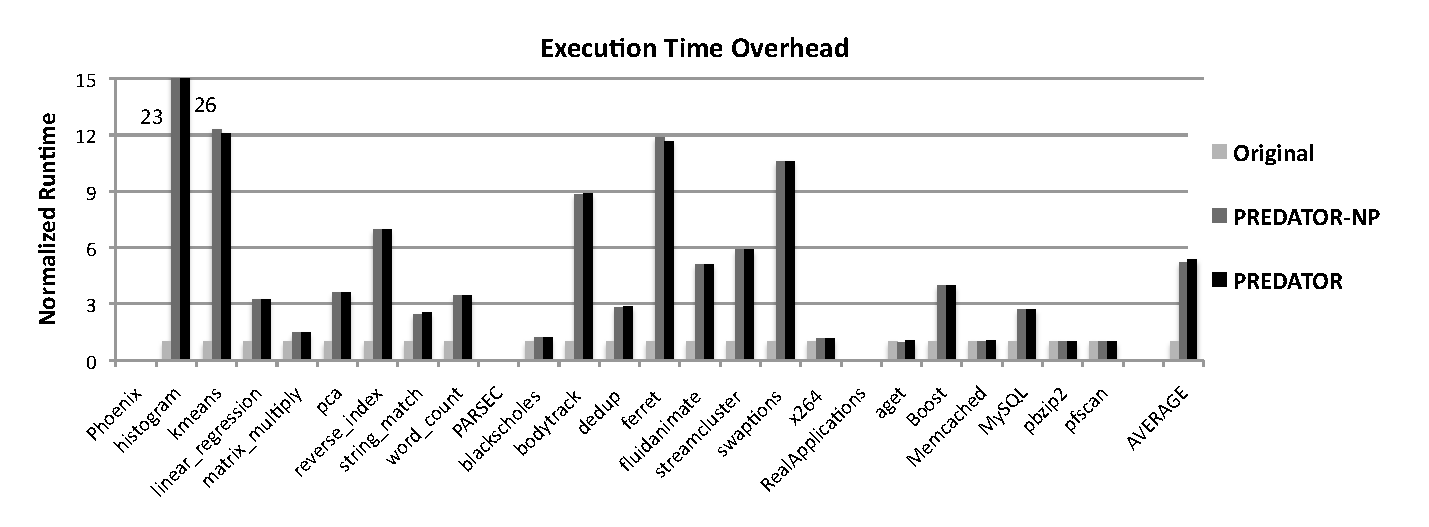
\includegraphics[width=6in]{fig/perf}
\caption{
Execution time overhead of \Predator{} with and without prediction (PREDATOR-NP).
\label{fig:perf}}
\end{figure*}


Figure~\ref{fig:perf} presents runtime overhead for using \Predator{}. All 
measurements are based on the average of $10$ runs, excluding the maximum and minimum values. \Predator{} imposes an average of $5.4\times$ performance overhead. There is no noticeable difference on performance whether the prediction mechanism is enabled or not. 

Five of these (histogram, kmeans, bodytrack, ferret, and swaptions), have more than $8\times$ performance overhead. The histogram benchmark runs more than $26\times$ slower because tracking detailed accesses to cache lines with false sharing exacerbates the false sharing effect (see Section~\ref{sec:sample}). Although bodytrack and ferret have no false sharing, \Predator{} detects numerous cache lines with writes that exceed the {\it TrackingThreshold}, causing it to track detailed access information. We have not identified the exact cause of \Predator{}'s high performance overhead for kmeans.

As expected, \Predator{} imposes relatively little overhead for I/O-bound applications (matrix\_multiply, blackscholes, x264, aget, Memcached, pbzip2, and pfscan).

\subsection{Memory Overhead}
\label{sec:memoverhead}

Figure~\ref{fig:memusage} and~\ref{fig:absolutememusage} present \Predator{}'s relative and absolute memory overhead, respectively. We compute \Predator{}'s physical memory consumption via the proportional set size (PSS) obtained from the \texttt{/proc/self/smaps} file~\cite{memusage}. We periodically collect this data and use the sum of all memory mappings as the total physical memory usage of running an application.

\Predator{} imposes less than 50\% memory overhead for 17 out of 22 applications.  For swaptions and aget, \Predator{} introduces high \emph{relative} memory overhead because their original memory footprints are extraordinarily small: both have sub-megabyte footprints. MySQL's increase in memory consumption, from 132 MB to 512 MB, is due to \Predator{}'s heap organization, which does not aggressively reclaim memory held by individual threads. In all cases where \Predator{}'s imposes substantial memory overhead, the applications continue to comfortably fit into RAM on modern platforms.

\subsection{Sensitivity to Different Sampling Rates}
\label{sec:sensitivity}

Section~\ref{sec:sample} describes \Predator{}'s sampling approach to reduce tracking overhead. This section evaluates the effect of different sampling rates on performance and effectiveness. Note that running an application with different sampling rates does not affect its memory usage.

The default sampling rate used by \Predator{} is 1\%. To test \Predator{}'s sensitivity to this choice, we evaluate performance on a representative subset of the benchmarks with two other sampling rates: 0.1\% and 10\%. Figure~\ref{fig:sample} presents the results. As expected, \Predator{} introduces lower performance overhead at lower sampling rates. Even when using the 0.1\% sampling rate, \Predator{} is still able to detect all false sharing problems reported here, although it reports a lower number of cache invalidations.

\begin{figure*}[!t]
\centering
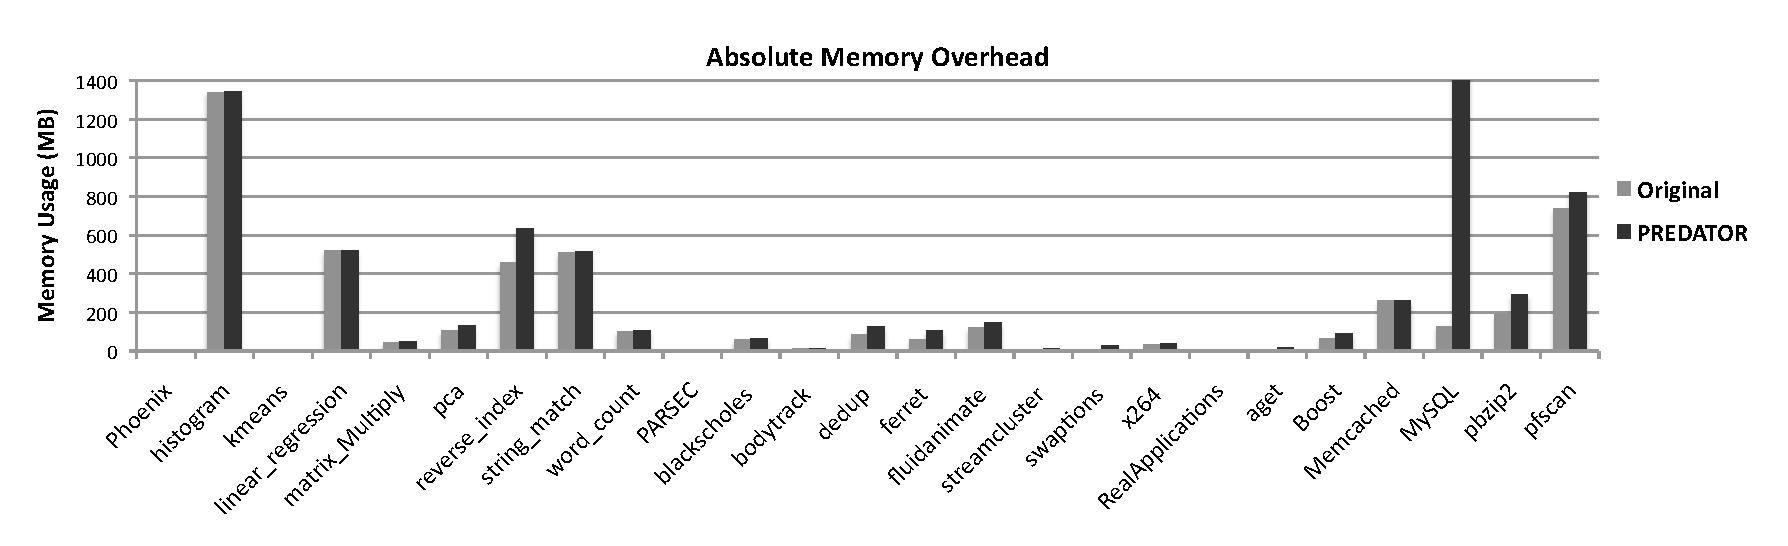
\includegraphics[width=6in]{fig/absolutememory}
\caption{Absolute physical memory usage overhead with \Predator{}.}
\label{fig:absolutememusage}
\end{figure*}

\begin{figure*}[!t]
\centering
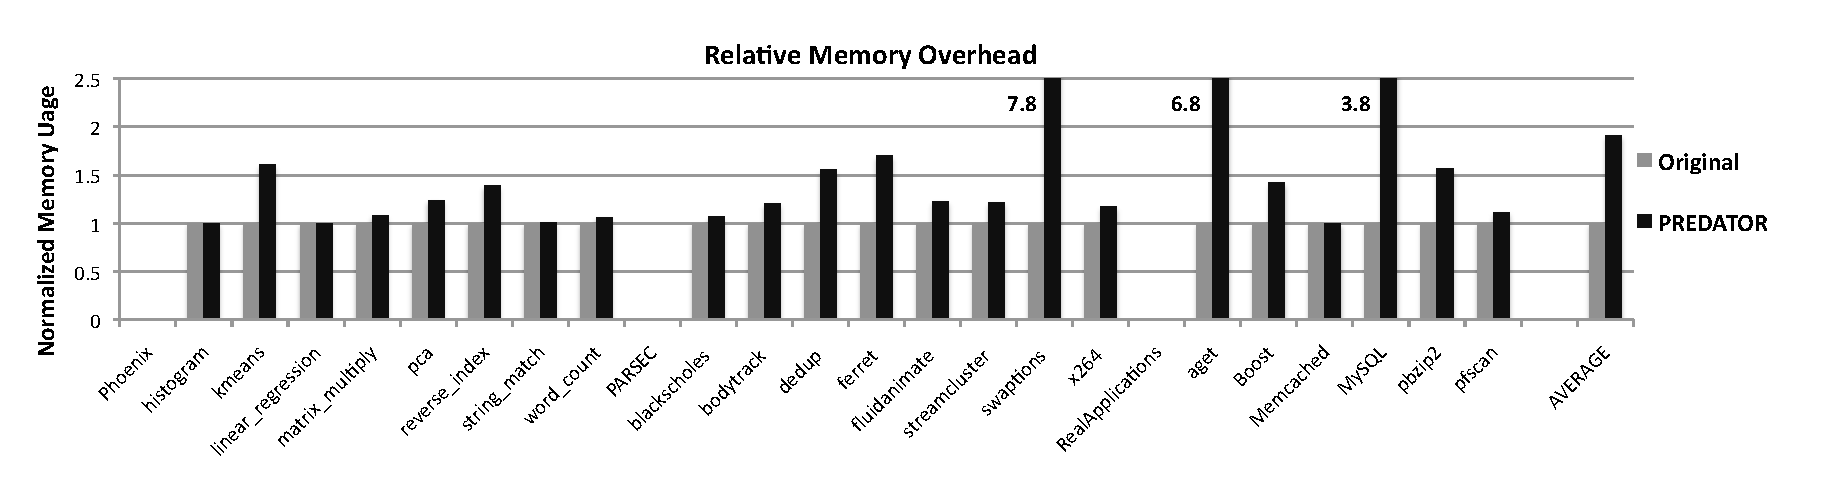
\includegraphics[width=6in]{fig/memusage}
\caption{Relative physical memory usage overhead with \Predator{}.}
\label{fig:memusage}
\end{figure*}

\section{Discussion}
\label{sec:discussion}

\subsection{Instrumentation Selection}
\label{sec:instrumentationtradeoff}
Dynamic binary instrumentation and compiler-based instrumentation are two alternative approaches for performing instrumentation~\cite{Instrumentation}. They exhibit different tradeoffs of performance and generality. Dynamic binary instrumentors, such as Valgrind~\cite{Valgrind}, Pin~\cite{Pin}, and DynamoRIO~\cite{DynamoRIO}, typically analyze the program's code just before execution in order to insert instrumentation. They introduce significant performance overhead, mostly caused by run-time encoding and decoding, but the fact that they operate directly on binaries makes them extremely convenient. By contrast, compiler instrumentation inserts instrumentation in the compilation phase, which requires re-compilation of all source code. 
\Predator{} employs compiler-based instrumentation both because of its better performance and its greater flexibility, as discussed in Section~\ref{sec:selectinstrumentation}.

\subsection{Effectiveness}
Several factors can affect \Predator{}'s ability to identify false sharing.

\begin{figure}[!t]
\centering 
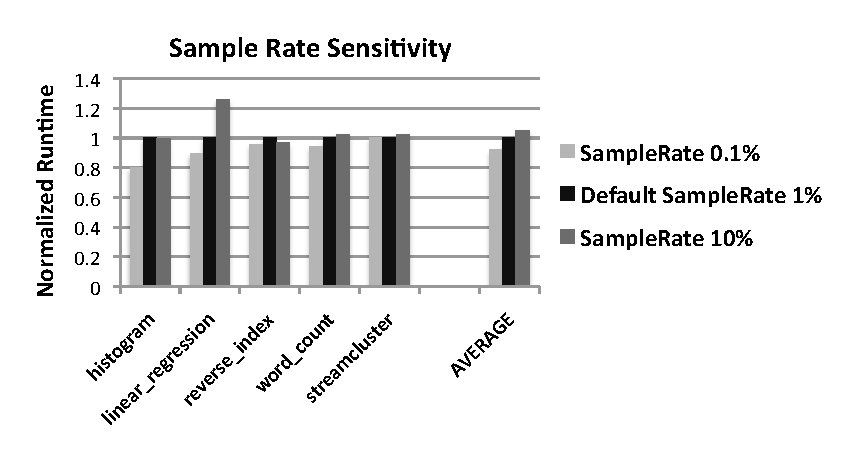
\includegraphics[width=3.4in]{fig/sample}
%\includegraphics{fig/potential.pdf}
\caption{Sampling rate sensitivity (execution time).}
\label{fig:sample}
\end{figure}

\paragraph{Different Inputs.} Different inputs trigger distinct executions of a program. If a specific input does not exercise the code with false sharing problems, \Predator{} cannot necessarily detect them. However, \Predator{} does generalize over inputs to find latent false sharing problems on those exercised code. When any reasonably representative set of inputs are exercised, as is required by any testing regime, \Predator{} can effectively predict false sharing.

\paragraph{Input Size.} Input size may affect detection results.  As discussed in Section~\ref{optimization}, \Predator{} introduces several threshold values to reduce tracking overhead, which can be adjusted as needed. If the input size is so small that it cannot generate enough false sharing events to cross the predefined thresholds, then the detection mechanism will not be triggered. In such cases, \Predator{} will miss actual cases of false sharing. However, realistically large inputs should be enough to trigger \Predator{}'s detection mechanisms. In our experience, running applications for at least 150 seconds is sufficient to expose false sharing problems. 

\paragraph{Hardware Independence.}  \Predator{}'s compiler-based approach make it independent of the underlying hardware platform. This approach increases generality, but may lead it to over-report false sharing. \Predator{} conservatively assumes that different threads are running on different cores and detects false sharing problems based on possible cache invalidations. However, if multiple threads involved in false sharing are on the same core, then there will be no performance impact. 

\section{Future Work}
\label{sec:futurework}

We have identified several directions along which \Predator{} could be enhanced.

\paragraph{Use Across the Software Stack.} 
\Predator{}'s architecture should in principle let it detect and predict false sharing in the entire software stack, including hypervisors, operating systems, libraries, and applications using different threading libraries.

\paragraph{Improved Performance.}
\Predator{} currently imposes approximately $6\times$ performance overhead. In the current implementation, every memory access is instrumented with a library call to notify the runtime system. A library call entails not only normal function call overhead but also Global Offset Table (GOT) and/or Procedure Linkage Table (PLT) lookup overhead. We plan to improve \Predator{}'s performance by inserting relevant code directly, rather than via function calls.

\paragraph{Suggest Fixes.} Finally, we would like to enhance \Predator{}'s reporting. We believe that leveraging memory trace information will make it possible for \Predator{} to prescribe fixes to the programmer to help them eliminate false sharing.


\section{Related Work}
\label{sec:relatedwork}

This section describes related work in detecting or preventing false sharing; no prior work predicts false sharing.

\subsection{False Sharing Detection}
Schindewolf et al.\ designed a tool based on the SIMICS functional simulator to report different kinds of cache usage information, such as cache misses and cache invalidations~\cite{falseshare:simulator}. Pluto relies on the Valgrind dynamic instrumentation framework to track the sequence of memory read and write events on different threads, and reports a worst-case estimation of possible false sharing~\cite{falseshare:binaryinstrumentation1}.
Similarly, Liu uses Pin to collect memory access information, and reports total cache miss information~\cite{falseshare:binaryinstrumentation2}.
These tools impose about $100-200\times$ performance overhead.

Zhao et al.\ present a tool based on the DynamoRIO framework to detect false sharing and other cache contention problems
for multithreading programs~\cite{qinzhaodetection}. 
It uses a shadow memory technique to maintain memory access history and detects cache invalidations based on the ownership of cache lines. However, it can only support at most $8$ threads. In addition, it cannot differentiate cold cache misses from actual false sharing problems.

Intel's performance tuning utility (PTU) uses Precise Event Based Sampling (PEBS) hardware support to detect false sharing problems~\cite{detect:ptu,detect:intel}.  PTU cannot distinguish true sharing from false sharing. In addition, PTU aggregates memory accesses without considering memory reuse and access interleavings, leading to numerous false positives. Sanath et al.\ designed a machine learning based approach to detect false sharing problems. They train their classifier on mini-programs and apply this classifier to general programs~\cite{mldetect}. Instead of instrumenting memory accesses, this tool relies on hardware performance counters to collect memory accesses events. This approach operates with extremely low overhead but ties false sharing detection to a specific hardware platform.

In addition to their individual disadvantages,
all approaches discussed above share a common shortcoming:  
they cannot pinpoint the exact location of false sharing in the source code, so programmers must manually examine the source code to identify problems.

Pesterev et al.\ present DProf, a tool that help programmers identify cache misses based on AMD's instruction-based sampling hardware~\cite{DProf}. DProf requires manual annotation to locate data types and object fields, and cannot detect false sharing when multiple objects reside on the same cache line.

\subsection{False Sharing Prevention}

Jeremiassen and Eggers use a compiler transformation to automatically adjust the memory layout of applications through padding and alignment~cite{falseshare:compile}. Chow et al.\ alter parallel loop scheduling in order to avoid false
sharing~\cite{falseshare:schedule}. These approaches only works for regular, array-based scientific code.

Berger et al.\ describe Hoard, a scalable memory allocator that can reduce the possibility of false sharing by making different threads use different heaps~\cite{Hoard}. Hoard cannot avoid false sharing problem in global variables or within a single heap object: the latter appears to be the primary source of false sharing problems.

\subsection{False Sharing Detection and Prevention}

\sheriff{} provides two tools to handle false sharing based on its ``threads-as-processes'' framework~\cite{sheriff}.
\Sheriff{}'s detection tool reports false sharing accurately and precisely with only $20\%$ performance overhead.
However, it can only detect write-write false sharing, and only works for programs that use the \pthreads{} library. It can also break programs that communicate across different threads with stack variables or \emph{ad hoc} synchronizations. These shortcomings limit \Sheriff{}'s usefulness for real-world applications.  
\Predator{} can detect all kinds of false sharing and imposes no limitations on the kind of applications it works on. 

\Sheriff{}'s prevention tool prevents false sharing altogether, eliminating the need for programmer intervention. However, in programs with many synchronization calls, the overhead imposed by \Sheriff{} could lead to performance degradation.

Plastic leverages the sub-page granularity memory remapping facility provided by the Xen hypervisor to detect and tolerate false sharing automatically~\cite{OSdetection}. However, the sub-page memory remapping mechanism is not currently supported by most existing operating systems, reducing its generality. In addition, Plastic cannot pinpoint the exact source of false sharing.  
In order to utilize Plastic's prevention tool, a program has to run on the Xen hypervisor, limiting the applicability of their prevention technique.

\section{Conclusion}
\label{sec:conclusion}
This paper introduces \emph{predictive false sharing detection}, and presents a prototype system that performs this detection called \Predator{}. By collecting and analyzing information through instrumented reads and writes, the runtime system detects false sharing based on cache invalidations and only reports those potentially causing severe performance degradation.
\Predator{} predicts potential false sharing that could be caused by a change of hardware cache line size or the starting addresses of objects. By identifying latent false sharing problems that can occur in the wild but which are unobserved in the test environment, \Predator{} overcomes a key limitation of
all previous false sharing detection approaches.

Our evaluation shows that \Predator{} can effectively detect and predict several previously unknown and existing false sharing problems in two popular benchmark suites, Phoenix and PARSEC. We also evaluate \Predator{} on six real applications. 
It successfully detects two known false sharing problems inside MySQL and the Boost library.
Fixing these false sharing problems improves performance by $6\times$ and $40\%$, respectively.

% Availability.

\acks
This material is based upon work supported by the National Science
Foundation under Grant No. 1012195-CCF. The authors thank Junjie Gu for his assistance with LLVM. The authors also thank Charlie Curtsinger, Dimitar Gochev, John Altidor and the anonymous reviewers for their helpful suggestions during the development of this work. Tongping Liu was supported by an internship while at Huawei US Research Center.

% The bibliography should be embedded for final submission.
\begin{thebibliography}{10}

\bibitem{Hoard}
E.~D. Berger, K.~S. McKinley, R.~D. Blumofe, and P.~R. Wilson.
\newblock Hoard: A scalable memory allocator for multithreaded applications.
\newblock In {\em Proceedings of the International Conference on Architectural
  Support for Programming Languages and Operating Systems (ASPLOS-IX)}, pages
  117--128, Cambridge, MA, Nov. 2000.

\bibitem{heaplayers}
E.~D. Berger, B.~G. Zorn, and K.~S. McKinley.
\newblock Composing high-performance memory allocators.
\newblock In {\em Proceedings of the ACM SIGPLAN 2001 conference on Programming
  language design and implementation}, PLDI '01, pages 114--124, New York, NY,
  USA, 2001. ACM.

\bibitem{parsec}
C.~Bienia and K.~Li.
\newblock {PARSEC} 2.0: A new benchmark suite for chip-multiprocessors.
\newblock In {\em Proceedings of the 5th Annual Workshop on Modeling,
  Benchmarking and Simulation}, June 2009.

\bibitem{falseshareeffect}
W.~J. Bolosky and M.~L. Scott.
\newblock False sharing and its effect on shared memory performance.
\newblock In {\em {SEDMS IV}: USENIX Symposium on Experiences with Distributed
  and Multiprocessor Systems}, pages 57--71, Berkeley, CA, USA, 1993. USENIX
  Association.

\bibitem{OSfalsesharing}
S.~Boyd-Wickizer, A.~T. Clements, Y.~Mao, A.~Pesterev, M.~F. Kaashoek,
  R.~Morris, and N.~Zeldovich.
\newblock An analysis of {Linux} scalability to many cores.
\newblock In {\em {Proceedings of the 9th USENIX Conference on Operating
  Systems Design and Implementation}}, OSDI'10, pages 1--8, Berkeley, CA, USA,
  2010. USENIX Association.

\bibitem{DynamoRIO}
D.~Bruening, T.~Garnett, and S.~Amarasinghe.
\newblock An infrastructure for adaptive dynamic optimization.
\newblock In {\em Proceedings of the international symposium on Code generation
  and optimization: feedback-directed and runtime optimization}, CGO '03, pages
  265--275, Washington, DC, USA, 2003. IEEE Computer Society.

\bibitem{falseshare:schedule}
J.-H. Chow and V.~Sarkar.
\newblock False sharing elimination by selection of runtime scheduling
  parameters.
\newblock In {\em ICPP '97: Proceedings of the international Conference on
  Parallel Processing}, pages 396--403, Washington, DC, USA, 1997. IEEE
  Computer Society.

\bibitem{JVMfalsesharing}
{David Dice}.
\newblock False sharing induced by card table marking.
\newblock
  \url{https://blogs.oracle.com/dave/entry/false_sharing_induced_by_card},
  February 2011.

\bibitem{falseshare:binaryinstrumentation1}
S.~M. G\"{u}nther and J.~Weidendorfer.
\newblock Assessing cache false sharing effects by dynamic binary
  instrumentation.
\newblock In {\em WBIA '09: Proceedings of the Workshop on Binary
  Instrumentation and Applications}, pages 26--33, New York, NY, USA, 2009.
  ACM.

\bibitem{detect:ptu}
{Intel Corporation}.
\newblock {\em Intel Performance Tuning Utility 3.2 Update}, November 2008.

\bibitem{detect:intel}
{Intel Corporation}.
\newblock Avoiding and identifying false sharing among threads.
\newblock
  \url{http://software.intel.com/en-us/articles/avoiding-and-identifying-false-sharing-among-threads/},
  February 2010.

\bibitem{Instrumentation}
T.~Iskhodzhanov, R.~Kleckner, and E.~Stepanov.
\newblock Combining compile-time and run-time instrumentation for testing
  tools.
\newblock {\em Programmnye produkty i sistemy}, 3:224--231, 2013.

\bibitem{mldetect}
S.~Jayasena, S.~Amarasinghe, A.~Abeyweera, G.~Amarasinghe, H.~De~Silva,
  S.~Rathnayake, X.~Meng, and Y.~Liu.
\newblock Detection of false sharing using machine learning.
\newblock In {\em Proceedings of {SC13}: International Conference for High
  Performance Computing, Networking, Storage and Analysis}, SC '13, pages
  30:1--30:9, New York, NY, USA, 2013. ACM.

\bibitem{memusage}
{Justin L.}
\newblock A way to determine a process's "real" memory usage, i.e. private
  dirty {RSS}?
\newblock
  \url{http://stackoverflow.com/questions/118307/a-way-to-determine-a-processs-real-memory-usage-i-e-private-dirty-rss},
  October 2011.

\bibitem{llvm}
C.~Lattner and V.~Adve.
\newblock {LLVM}: A compilation framework for lifelong program analysis \&
  transformation.
\newblock In {\em Proceedings of the International Symposium on Code Generation
  and Optimization: Feedback-directed and Runtime Optimization}, CGO '04, pages
  75--, Washington, DC, USA, 2004. IEEE Computer Society.

\bibitem{falseshare:binaryinstrumentation2}
C.-L. Liu.
\newblock False sharing analysis for multithreaded programs.
\newblock Master's thesis, National Chung Cheng University, July 2009.

\bibitem{sheriff}
T.~Liu and E.~D. Berger.
\newblock \textsc{Sheriff}: Precise detection and automatic mitigation of false
  sharing.
\newblock In {\em {Proceedings of the 2011 ACM International Conference on
  Object-Oriented Programming Systems Languages and Applications}}, OOPSLA '11,
  pages 3--18, New York, NY, USA, 2011. ACM.

\bibitem{Pin}
C.-K. Luk, R.~Cohn, R.~Muth, H.~Patil, A.~Klauser, G.~Lowney, S.~Wallace, V.~J.
  Reddi, and K.~Hazelwood.
\newblock Pin: Building customized program analysis tools with dynamic
  instrumentation.
\newblock In {\em Proceedings of the 2005 ACM SIGPLAN Conference on Programming
  Language Design and Implementation}, PLDI '05, pages 190--200, New York, NY,
  USA, 2005. ACM.

\bibitem{libfalsesharing}
{mcmcc}.
\newblock False sharing in boost::detail::spinlock pool?
\newblock
  \url{http://stackoverflow.com/questions/11037655/false-sharing-in-boostdetailspinlock-pool},
  June 2012.

\bibitem{mysql}
{Mikael Ronstrom}.
\newblock Mysql team increases scalability by >50% for sysbench oltp ro in
  mysql 5.6 labs release april 2012.
\newblock
  \url{http://mikaelronstrom.blogspot.com/2012/04/mysql-team-increases-scalability-by-50.html},
  April 2012.

\bibitem{OSdetection}
M.~Nanavati, M.~Spear, N.~Taylor, S.~Rajagopalan, D.~T. Meyer, W.~Aiello, and
  A.~Warfield.
\newblock Whose cache line is it anyway?: operating system support for live
  detection and repair of false sharing.
\newblock In {\em Proceedings of the 8th ACM European Conference on Computer
  Systems}, EuroSys '13, pages 141--154, New York, NY, USA, 2013. ACM.

\bibitem{Valgrind}
N.~Nethercote and J.~Seward.
\newblock Valgrind: a framework for heavyweight dynamic binary instrumentation.
\newblock In {\em Proceedings of the 2007 ACM SIGPLAN conference on Programming
  language design and implementation}, PLDI '07, pages 89--100, New York, NY,
  USA, 2007. ACM.

\bibitem{appfalsesharing}
K.~Papadimitriou.
\newblock Taming false sharing in parallel programs.
\newblock Master's thesis, University of Edinburgh, 2009.

\bibitem{DProf}
A.~Pesterev, N.~Zeldovich, and R.~T. Morris.
\newblock Locating cache performance bottlenecks using data profiling.
\newblock In {\em EuroSys '10: Proceedings of the 5th European conference on
  Computer systems}, pages 335--348, New York, NY, USA, 2010. ACM.

\bibitem{phoenix-hpca}
C.~Ranger, R.~Raghuraman, A.~Penmetsa, G.~Bradski, and C.~Kozyrakis.
\newblock Evaluating {MapReduce} for multi-core and multiprocessor systems.
\newblock In {\em HPCA '07: Proceedings of the 2007 IEEE 13th International
  Symposium on High Performance Computer Architecture}, pages 13--24,
  Washington, DC, USA, 2007. IEEE Computer Society.

\bibitem{falseshare:simulator}
M.~Schindewolf.
\newblock Analysis of cache misses using {SIMICS}.
\newblock Master's thesis, Institute for Computing Systems Architecture,
  University of Edinburgh, 2007.

\bibitem{Addresssanitizer}
K.~Serebryany, D.~Bruening, A.~Potapenko, and D.~Vyukov.
\newblock {AddressSanitizer}: a fast address sanity checker.
\newblock In {\em Proceedings of the 2012 {USENIX} Annual Technical
  Conference}, USENIX ATC'12, pages 28--28, Berkeley, CA, USA, 2012. USENIX
  Association.

\bibitem{qinzhaodetection}
Q.~Zhao, D.~Koh, S.~Raza, D.~Bruening, W.-F. Wong, and S.~Amarasinghe.
\newblock Dynamic cache contention detection in multi-threaded applications.
\newblock In {\em The International Conference on Virtual Execution
  Environments}, Newport Beach, CA, Mar 2011.

\end{thebibliography}

%\begin{thebibliography}{}
%\end{thebibliography}

\end{document}
